\begin{boxE}
 \lr{
 \lstinputlisting[language=Python]{IR5/code/job_2.py}
 }   
\end{boxE}

\begin{figure}
    \centering
    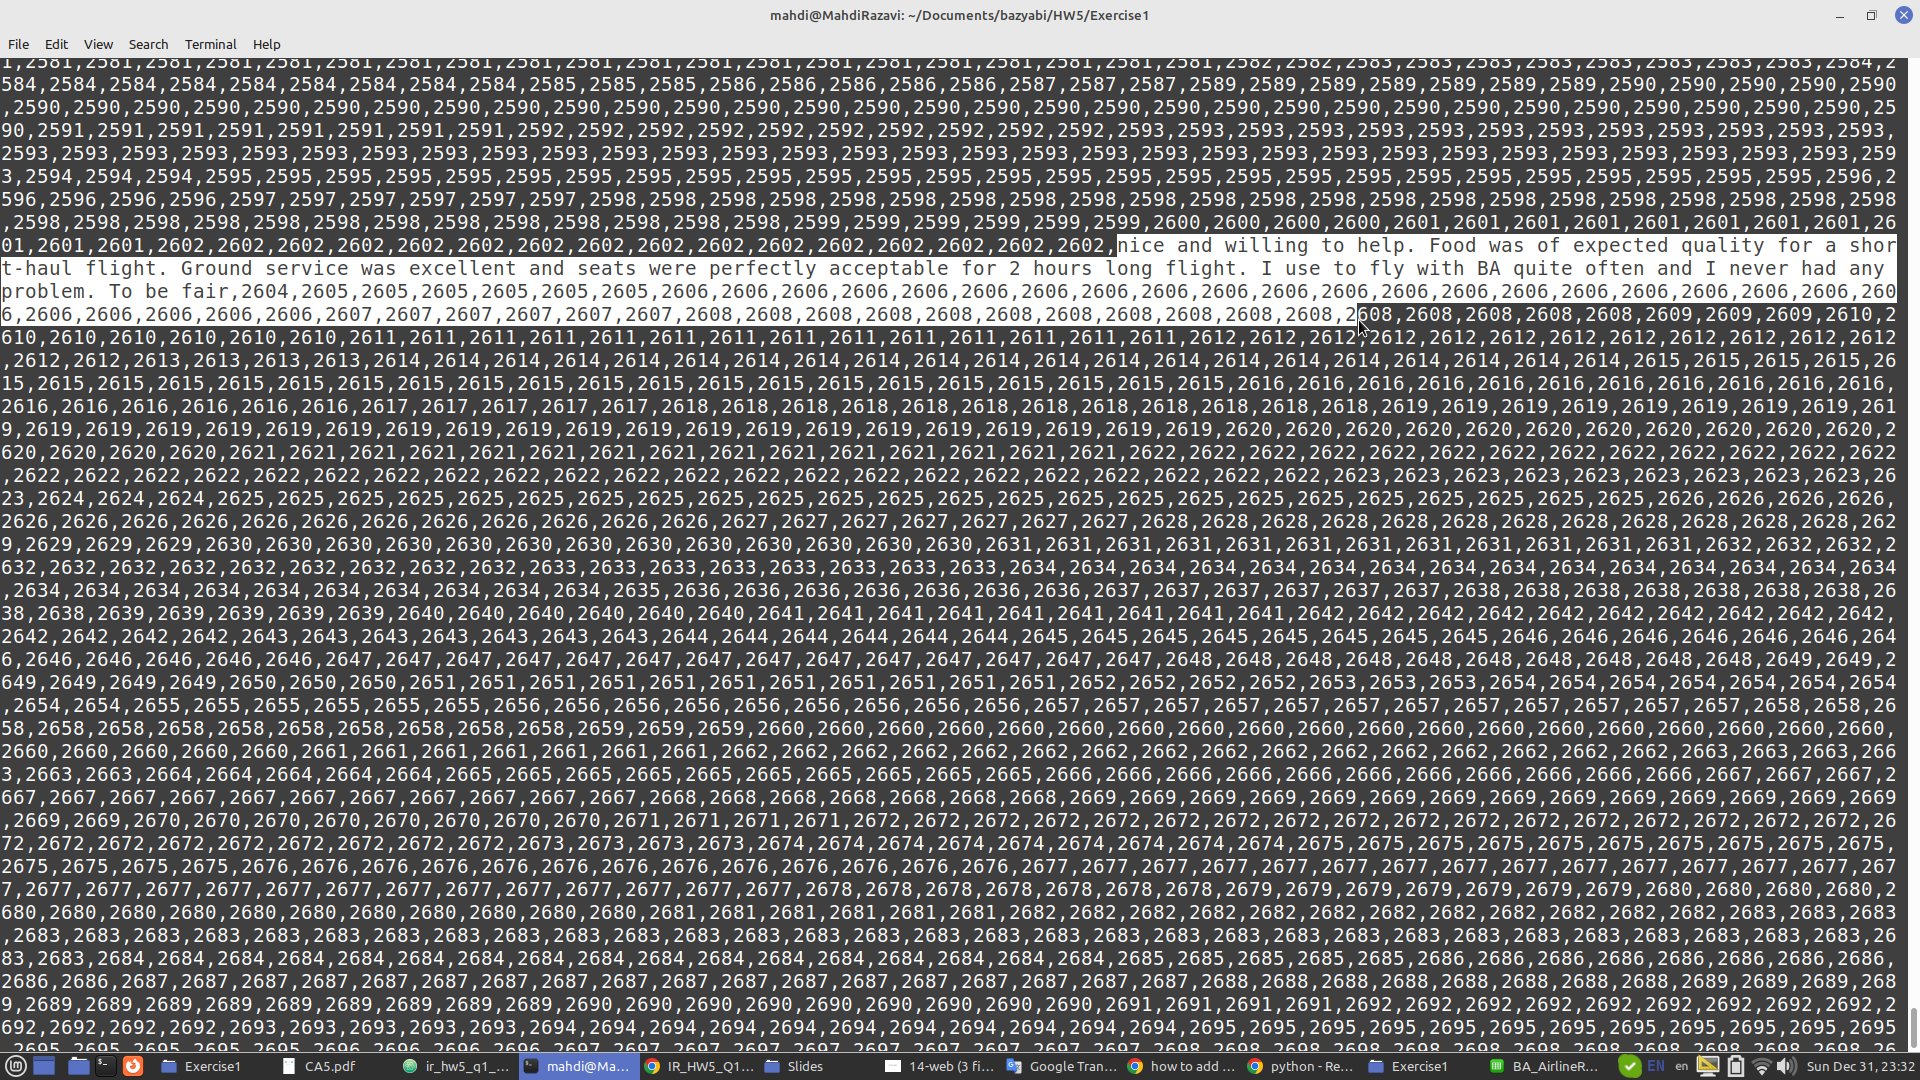
\includegraphics
    [width = 0.9\textwidth]
    {IR5/image/MapReduce2.png}
    \caption{
    استفاده از اندیس بازخورد برای ایجاد یک لیست شاخص معکوس برای کلمات موجود در بازخوردها
    }
    % \caption{نتایج حاصل از اجرای کد برای شمارش میزان نظرات تایید شده و تایید نشده}
    \label{fig:enter-label}
\end{figure}

\begin{boxM}
    % توضیحات نوشته شود.
    در گام
    \lr{Mapper}
    می‌بایستی هر کلمه موجود را به کد سند (ایندکس) نظیر کنیم.

    سپس در گام 
    \lr{Reducer}
    تابع
    \lr{Aggregator}
    % در واق
    ما در واقع
    \lr{Join}
    بر روی همه ایندکس‌ها خواهد بود
\end{boxM}